\chapter{Arhitektura i dizajn sustava}
		
		\textbf{\textit{dio 1. revizije}}\\

		\textit{ Potrebno je opisati stil arhitekture te identificirati: podsustave, preslikavanje na radnu platformu, spremišta podataka, mrežne protokole, globalni upravljački tok i sklopovsko-programske zahtjeve. Po točkama razraditi i popratiti odgovarajućim skicama:}
	\begin{itemize}
		\item 	\textit{izbor arhitekture temeljem principa oblikovanja pokazanih na predavanjima (objasniti zašto ste baš odabrali takvu arhitekturu)}
		\\Za razvoj frontend-a odabrali smo programski jezik TypeScript u kojem smo koristili React i React router biblioteku. To nam omogućuje razvoj stranice uz pomoć tzv. komponenti što čini kod čitljivije i dopušta lakše ponovno korištenje komponenti. Za izgled stranice koristili smo Bootstrap kako bi stranica imala moderan izgled. 
		
		\item 	\textit{organizaciju sustava s najviše razine apstrakcije (npr. klijent-poslužitelj, baza podataka, datotečni sustav, grafičko sučelje)}
		\\Ulaskom na stranicu korisnik (administrator) je preusmjeren na stranicu za prijavu. Nakon unosa svog korisničkog imena i lozinke, podatci se provjeravaju u bazi podataka, i ako su ispravni, administratora se  preusmjerava na glavnu stranicu. Na glavnoj stranici su prikazani
		različiti "prozori" ovisno o tome koja vrsta administratora pristupa stranici.
		\item 	\textit{organizaciju aplikacije (npr. slojevi frontend i backend, MVC arhitektura) }		
	\end{itemize}

	

		

				
		\section{Baza podataka}
			
			\textbf{\textit{dio 1. revizije}}\\
			
		\textit{Potrebno je opisati koju vrstu i implementaciju baze podataka ste odabrali, glavne komponente od kojih se sastoji i slično.}\\
		
		{Baza podataka modelirana je tabličnim modelom u "Structured Query Language" (SQL) jeziku. Ona sadrži podatke potrebne za rad cijelog sustava, poput podatke o administratorima, korisnicima, kao i podatke o vozilima koji su na raspolaganju te koji ih vozači voze, zajedno s adresama svih lokacija i vlasništva dostupnog smještaja.}
		
			\subsection{Opis tablica}
			
				
				{Entitet \textbf{Korisnik} sadržava informacije o korisniku. Atributi od kojih se sastoji entitet su: IDKor koji je ujedno i identifikacijski ključ korisnika,
				Ime, Prezime, DatDol odnosno vrijeme dolaska, DatOdl vrijeme odlaska, IdSmj, RegVoz i OdvoziRez. Ovaj entitet je u vezi One-to-One s entitetom  Smještaj preko atibuta
				IDSmj, te je u vezi One-to-One s entitetom Vozilo preko atributa RegVoz i OdlaziRegVoz.}
				
				\begin{longtblr}[
					label=none,
					entry=none
					]{
						width = \textwidth,
						colspec={|X[6,l]|X[6, l]|X[20, l]|}, 
						rowhead = 1,
					} %definicija širine tablice, širine stupaca, poravnanje i broja redaka naslova tablice
					\hline \SetCell[c=3]{c}{\textbf{Korisnik}}	 \\ \hline[3pt]
					\SetCell{LightGreen}IDKor & INT	&  	Identifikacijski ključ korinika	\\ \hline
					Ime	& VARCHAR & Ime korisnika  	\\ \hline 
					Prezime & VARCHAR &  Prezime korisnika \\ \hline 
					DatDol & TIMESTAMP	&  Datum dolaska korisnika		\\ \hline 
					DatOdl & TIMESTAMP	&  Datum odlaska korisnika		\\ \hline 
					\SetCell{LightBlue}IdSmj & INT	&  Identifikacijski ključ smještaja		\\ \hline 
					\SetCell{LightBlue}RegVozila & VARCHAR	& Identifikacijski ključ vozila u dolasku		\\ \hline 
					\SetCell{LightBlue}OdvoziReg	& VARCHAR & Identifikacijski ključ vozila u odlasku 	\\ \hline 
				\end{longtblr}
				
				{Entitet \textbf{Smještaj} opisuje smještaj u kojem će boraviti korisik. Sadrži atribute: IDSmj (ujedno i identifikacijski ključ), vrsta smještaja te IDAdr. Entitet Smještaj povezan je sa
				vezom Many-to-Many s entitetom Adresa preko	atributa IDAdr.}
				
				\begin{longtblr}[
					label=none,
					entry=none
					]{
						width = \textwidth,
						colspec={|X[6,l]|X[6, l]|X[20, l]|}, 
						rowhead = 1,
					} %definicija širine tablice, širine stupaca, poravnanje i broja redaka naslova tablice
					\hline \SetCell[c=3]{c}{\textbf{Smještaj}}	 \\ \hline[3pt]
					\SetCell{LightGreen}IDSmj & INT	&  	Identifikacijski ključ smještaja	\\ \hline
					Vrsta	& VARCHAR & Vrsta smještaja  	\\ \hline 
					\SetCell{LightBlue}IDAdr	& INT & Identifikacijski ključ adrese smještaja 	\\ \hline 
				\end{longtblr}
				
				{Entitet \textbf{Adresa} govori o samoj adresi smještaja i to s atributima: IDAdr, Mjesto, Ulica i Broj. Identifikacijski ključ ovog entiteta je IDAdr.}
				
				\begin{longtblr}[
					label=none,
					entry=none
					]{
						width = \textwidth,
						colspec={|X[6,l]|X[6, l]|X[20, l]|}, 
						rowhead = 1,
					} %definicija širine tablice, širine stupaca, poravnanje i broja redaka naslova tablice
					\hline \SetCell[c=3]{c}{\textbf{Adresa}}	 \\ \hline[3pt]
					\SetCell{LightGreen}IDAdr & INT	&  	Identifikacijski ključ adrese	\\ \hline
					Mjesto	& VARCHAR & Mjesto u adresi smještaja	\\ \hline 
					Ulica	& VARCHAR & Ulica u adresi smještaja	\\ \hline 
					Broj	& INT & Kućni broj u adresi smještaja	\\ \hline  
				\end{longtblr}


				{Entitet \textbf{Vozilo} sadrži informacije o samom vozilu. Sadrži atribute: RegVozila (registracija vozila), Model i Boja. Identifikacijski ključ entiteta je registracija vzila (RegVoz)}
				
				\begin{longtblr}[
					label=none,
					entry=none
					]{
						width = \textwidth,
						colspec={|X[6,l]|X[6, l]|X[20, l]|}, 
						rowhead = 1,
					} %definicija širine tablice, širine stupaca, poravnanje i broja redaka naslova tablice
					\hline \SetCell[c=3]{c}{\textbf{Vozilo}}	 \\ \hline[3pt]
					\SetCell{LightGreen}RegVozila & VARCHAR	&  	Identifikacijski ključ vozila	\\ \hline
					Model	& VARCHAR & Model vozila	\\ \hline 
					Boja	& VARCHAR & Boja vozila	\\ \hline 
				\end{longtblr}

				{Entitet \textbf{Vozač} opisuje vozača koji vozi i odvozi korisnika u i iz njegovog privremenog smještaja. Sadrži atribute: IDVoz (identifikacijski ključ), Ime, Prezime, Brradsat(broj radnih sati) te Regvozila. Povezan je s entitetom Vozilo sa vezom Many-to-Many preko atributa RegVozila.}
				
				\begin{longtblr}[
					label=none,
					entry=none
					]{
						width = \textwidth,
						colspec={|X[6,l]|X[6, l]|X[20, l]|}, 
						rowhead = 1,
					} %definicija širine tablice, širine stupaca, poravnanje i broja redaka naslova tablice
					\hline \SetCell[c=3]{c}{\textbf{Vozač}}	 \\ \hline[3pt]
					\SetCell{LightGreen}IDVoz & INT	&  	Identifikacijski ključ vožača	\\ \hline
					Ime	& VARCHAR & Ime vozača	\\ \hline 
					Prezime	& VARCHAR & Prezime vozača	\\ \hline
					Brradsat	& INT & Broj radnih sati vozača	\\ \hline  
					\SetCell{LightBlue}RegVozila	& VARCHAR & Identifikacijski ključ vozila 	\\ \hline
				\end{longtblr}

				{Entitet \textbf{Admin} sadrži informacije o adminu profilu te se sastoji od artibuta: UserName i lozinka.}
				
				\begin{longtblr}[
					label=none,
					entry=none
					]{
						width = \textwidth,
						colspec={|X[6,l]|X[6, l]|X[20, l]|}, 
						rowhead = 1,
					} %definicija širine tablice, širine stupaca, poravnanje i broja redaka naslova tablice
					\hline \SetCell[c=3]{c}{\textbf{Admin}}	 \\ \hline[3pt]
					\SetCell{LightGreen}UserName & VARCHAR	&  	Identifikacijski ključ admina	\\ \hline
					Lozinka	& VARCHAR & Lozinka admina	\\ \hline 
					\end{longtblr}
			
				{Entitet \textbf{AdminUloga} povezuje admina s njegovom ulogom. Sastoji se od atributa: UserName i IDUloge. Povezan je s entitetom Admin s vezom Many-to-Many te preko atributa UserName, te je spojen također s vezom Many-to-Many s entiteom Uloge preko atributa IDUloge.}
				
				\begin{longtblr}[
					label=none,
					entry=none
					]{
						width = \textwidth,
						colspec={|X[6,l]|X[6, l]|X[20, l]|}, 
						rowhead = 1,
					} %definicija širine tablice, širine stupaca, poravnanje i broja redaka naslova tablice
					\hline \SetCell[c=3]{c}{\textbf{AdminUloga}}	 \\ \hline[3pt]
					\SetCell{LightBlue}UserName	& VARCHAR & Orisničko ime admina 	\\ \hline
					\SetCell{LightBlue}IDUloge	& VARCHAR & ID Uloge admina	\\ \hline
					\end{longtblr}

				{Entitet \textbf{Uloge} sadrži informacije o samoj ulozi. Aributi od kojij se sastoji su: IDUloge(identifikacijski ključ) te Uloga}
				
				\begin{longtblr}[
					label=none,
					entry=none
					]{
						width = \textwidth,
						colspec={|X[6,l]|X[6, l]|X[20, l]|}, 
						rowhead = 1,
					} %definicija širine tablice, širine stupaca, poravnanje i broja redaka naslova tablice
					\hline \SetCell[c=3]{c}{\textbf{Uloge}}	 \\ \hline[3pt]
					\SetCell{LightGreen}IDUloge & VARCHAR	&  	Identifikacijski ključ uloge admina	\\ \hline
					Uloga	& VARCHAR & Uloga admina	\\ \hline 
					\end{longtblr}

			\subsection{Dijagram baze podataka}
				\textit{ U ovom potpoglavlju potrebno je umetnuti dijagram baze podataka. Primarni i strani ključevi moraju biti označeni, a tablice povezane. Bazu podataka je potrebno normalizirati. Podsjetite se kolegija "Baze podataka".}
			
			
			\begin{figure}[H]
				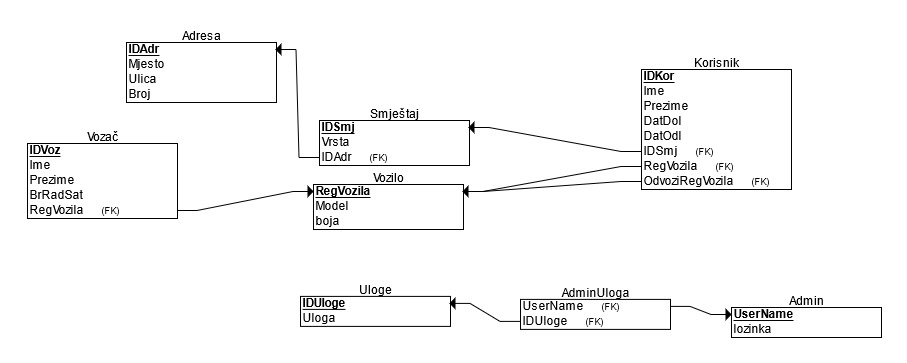
\includegraphics[width=\linewidth]{slike/DentAll_RelacijskiDijagramBaze.png}
				\centering
				\caption{Dijagram baze podataka}
				\label{fig:dijagramBaze}
			\end{figure}
			\eject
			
		\section{Dijagram razreda}
		
			{Na sljedećim slikama prikazani su dijagrami razreda koji se odnose na \textit{backend} dio aplikacije. Na slici 4.1 prikazan je cjelokupni dijagram razreda, a na ostalima su razdvojeni u smislene cjeline. U implementaciji korištena je \textit{Spring Boot} tehnologija. Postoje tri sloja aplikacije: \textit{Controller}(REST API), \textit{Service}(poslovna logika) te \textit{Repository}(pristup podacima). }\\
			
			\begin{figure}[H]
				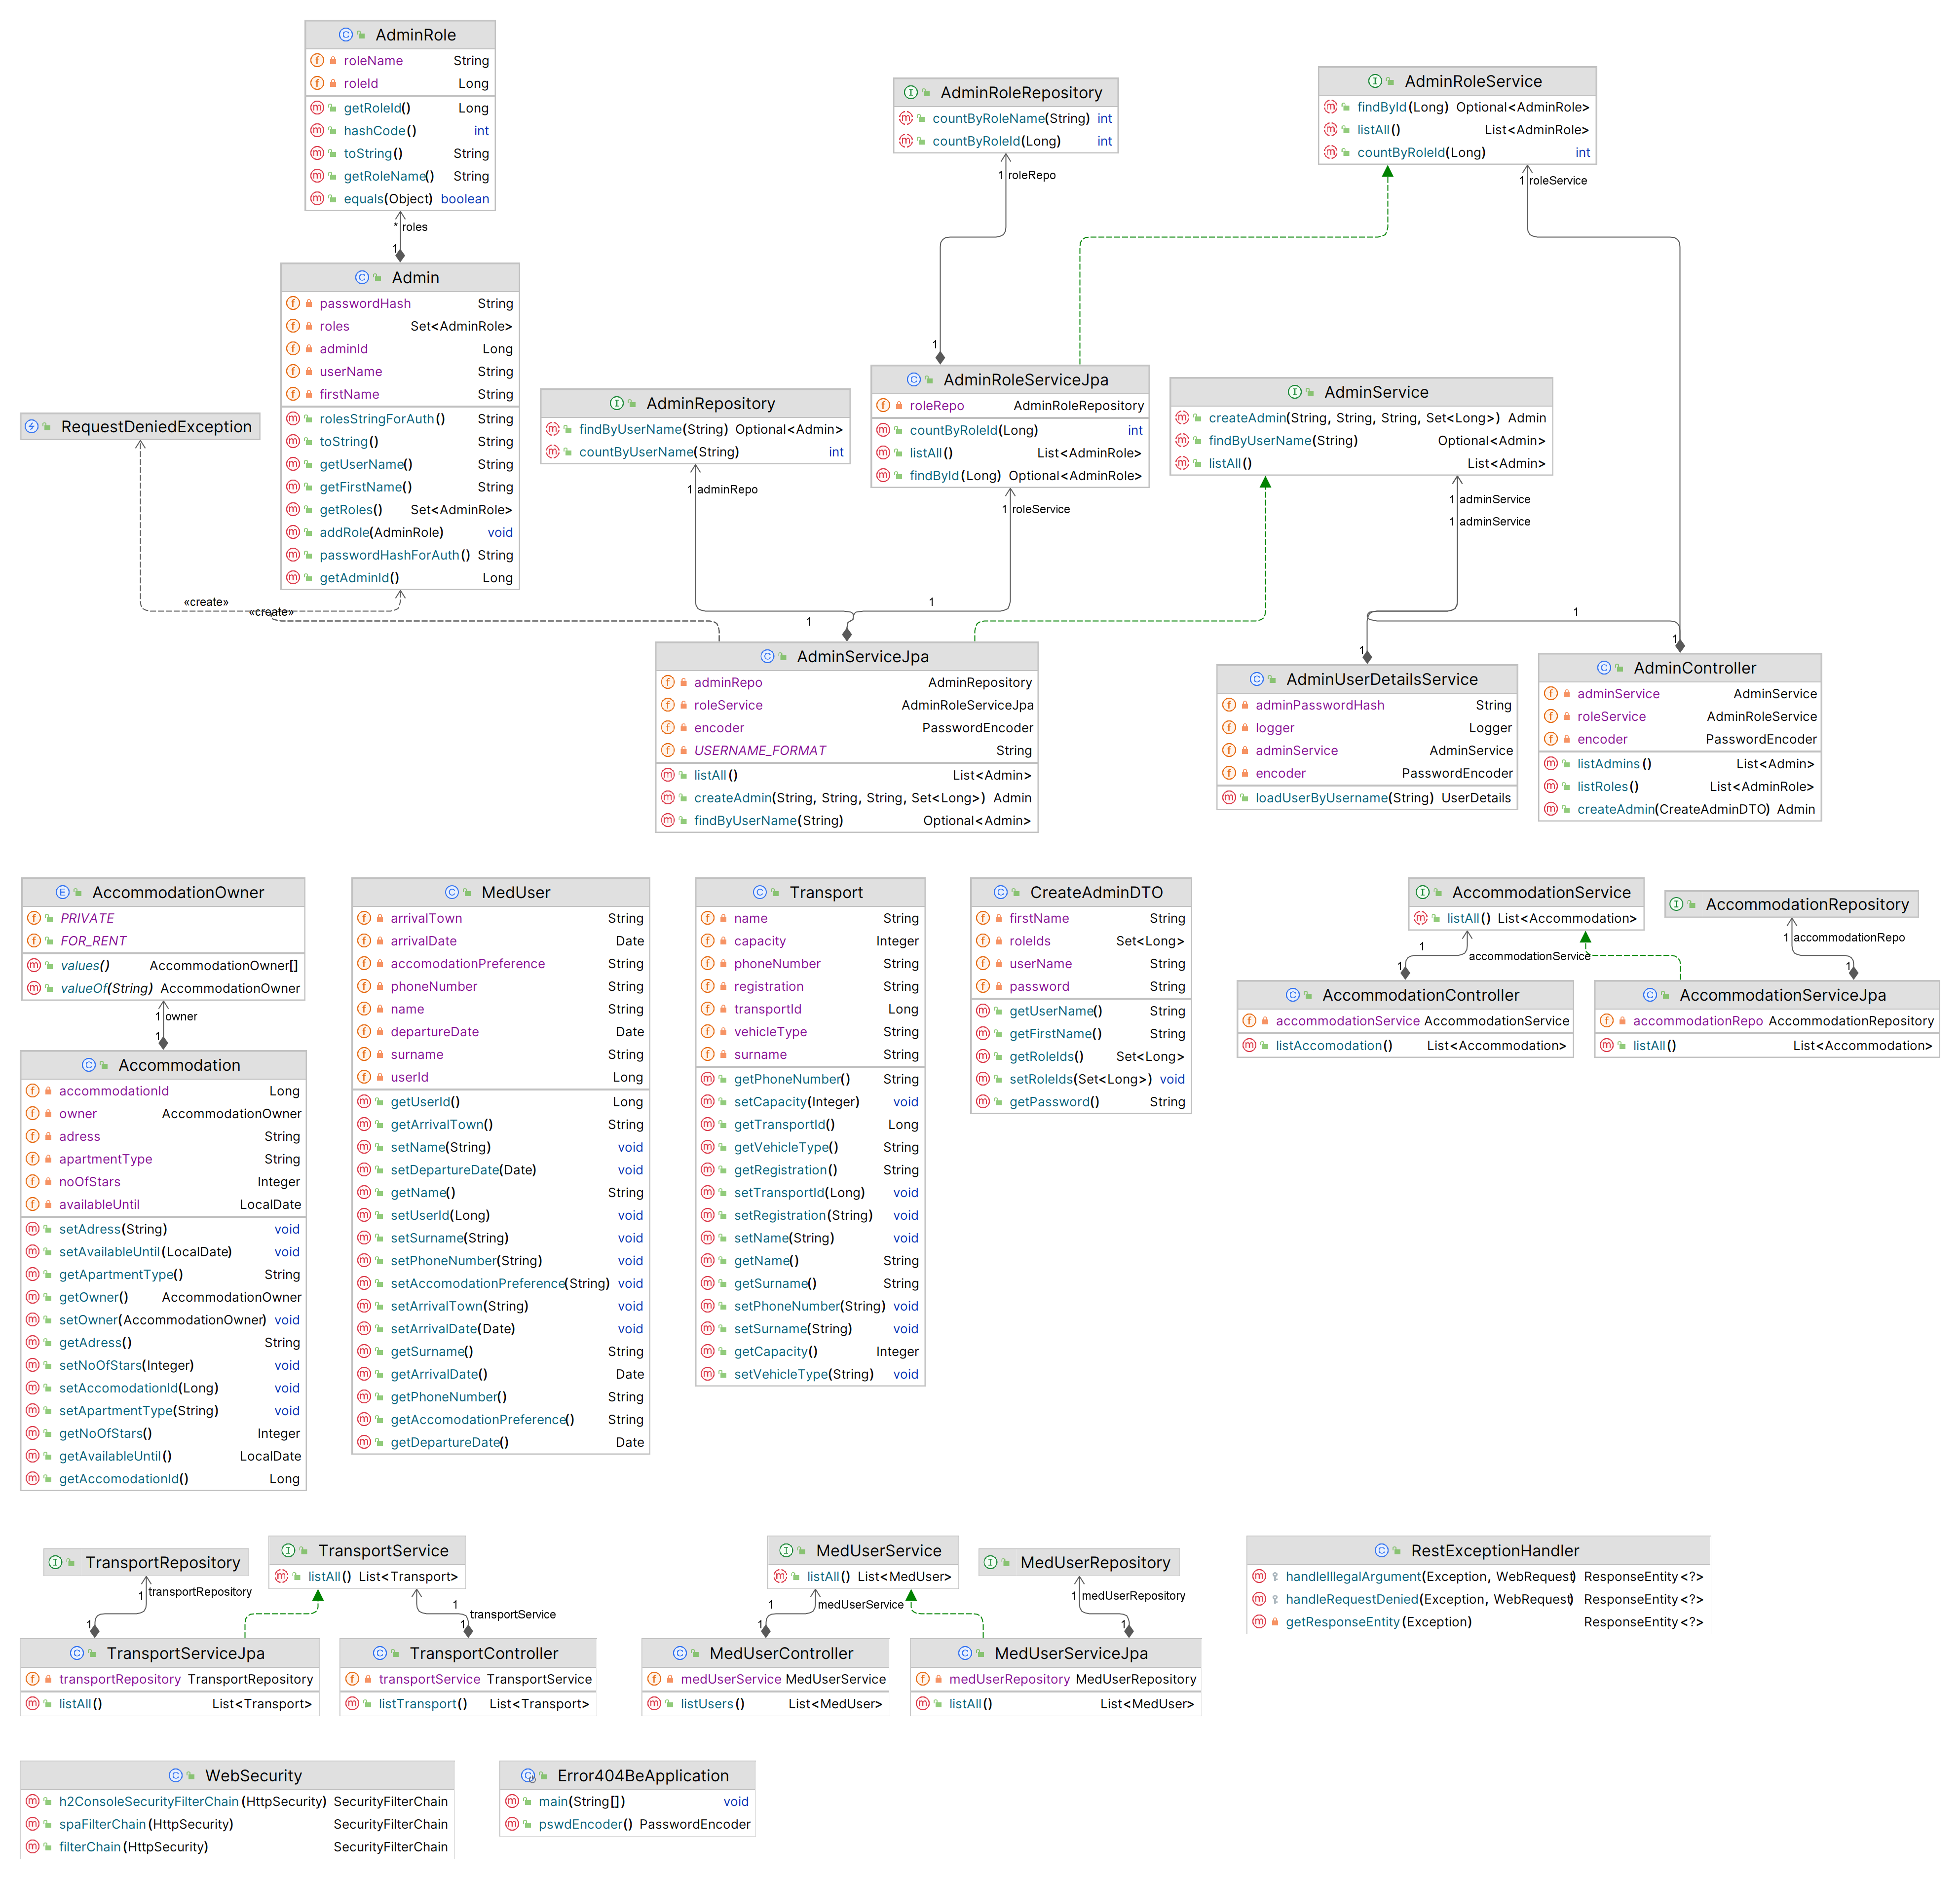
\includegraphics[width=\textwidth]{slike/CjelokupanDijagramRazreda.PNG}
				\caption{Cjelokupan dijagram razreda}
				\label{classDiagram}
			\end{figure}
			
			\begin{figure}[H]
				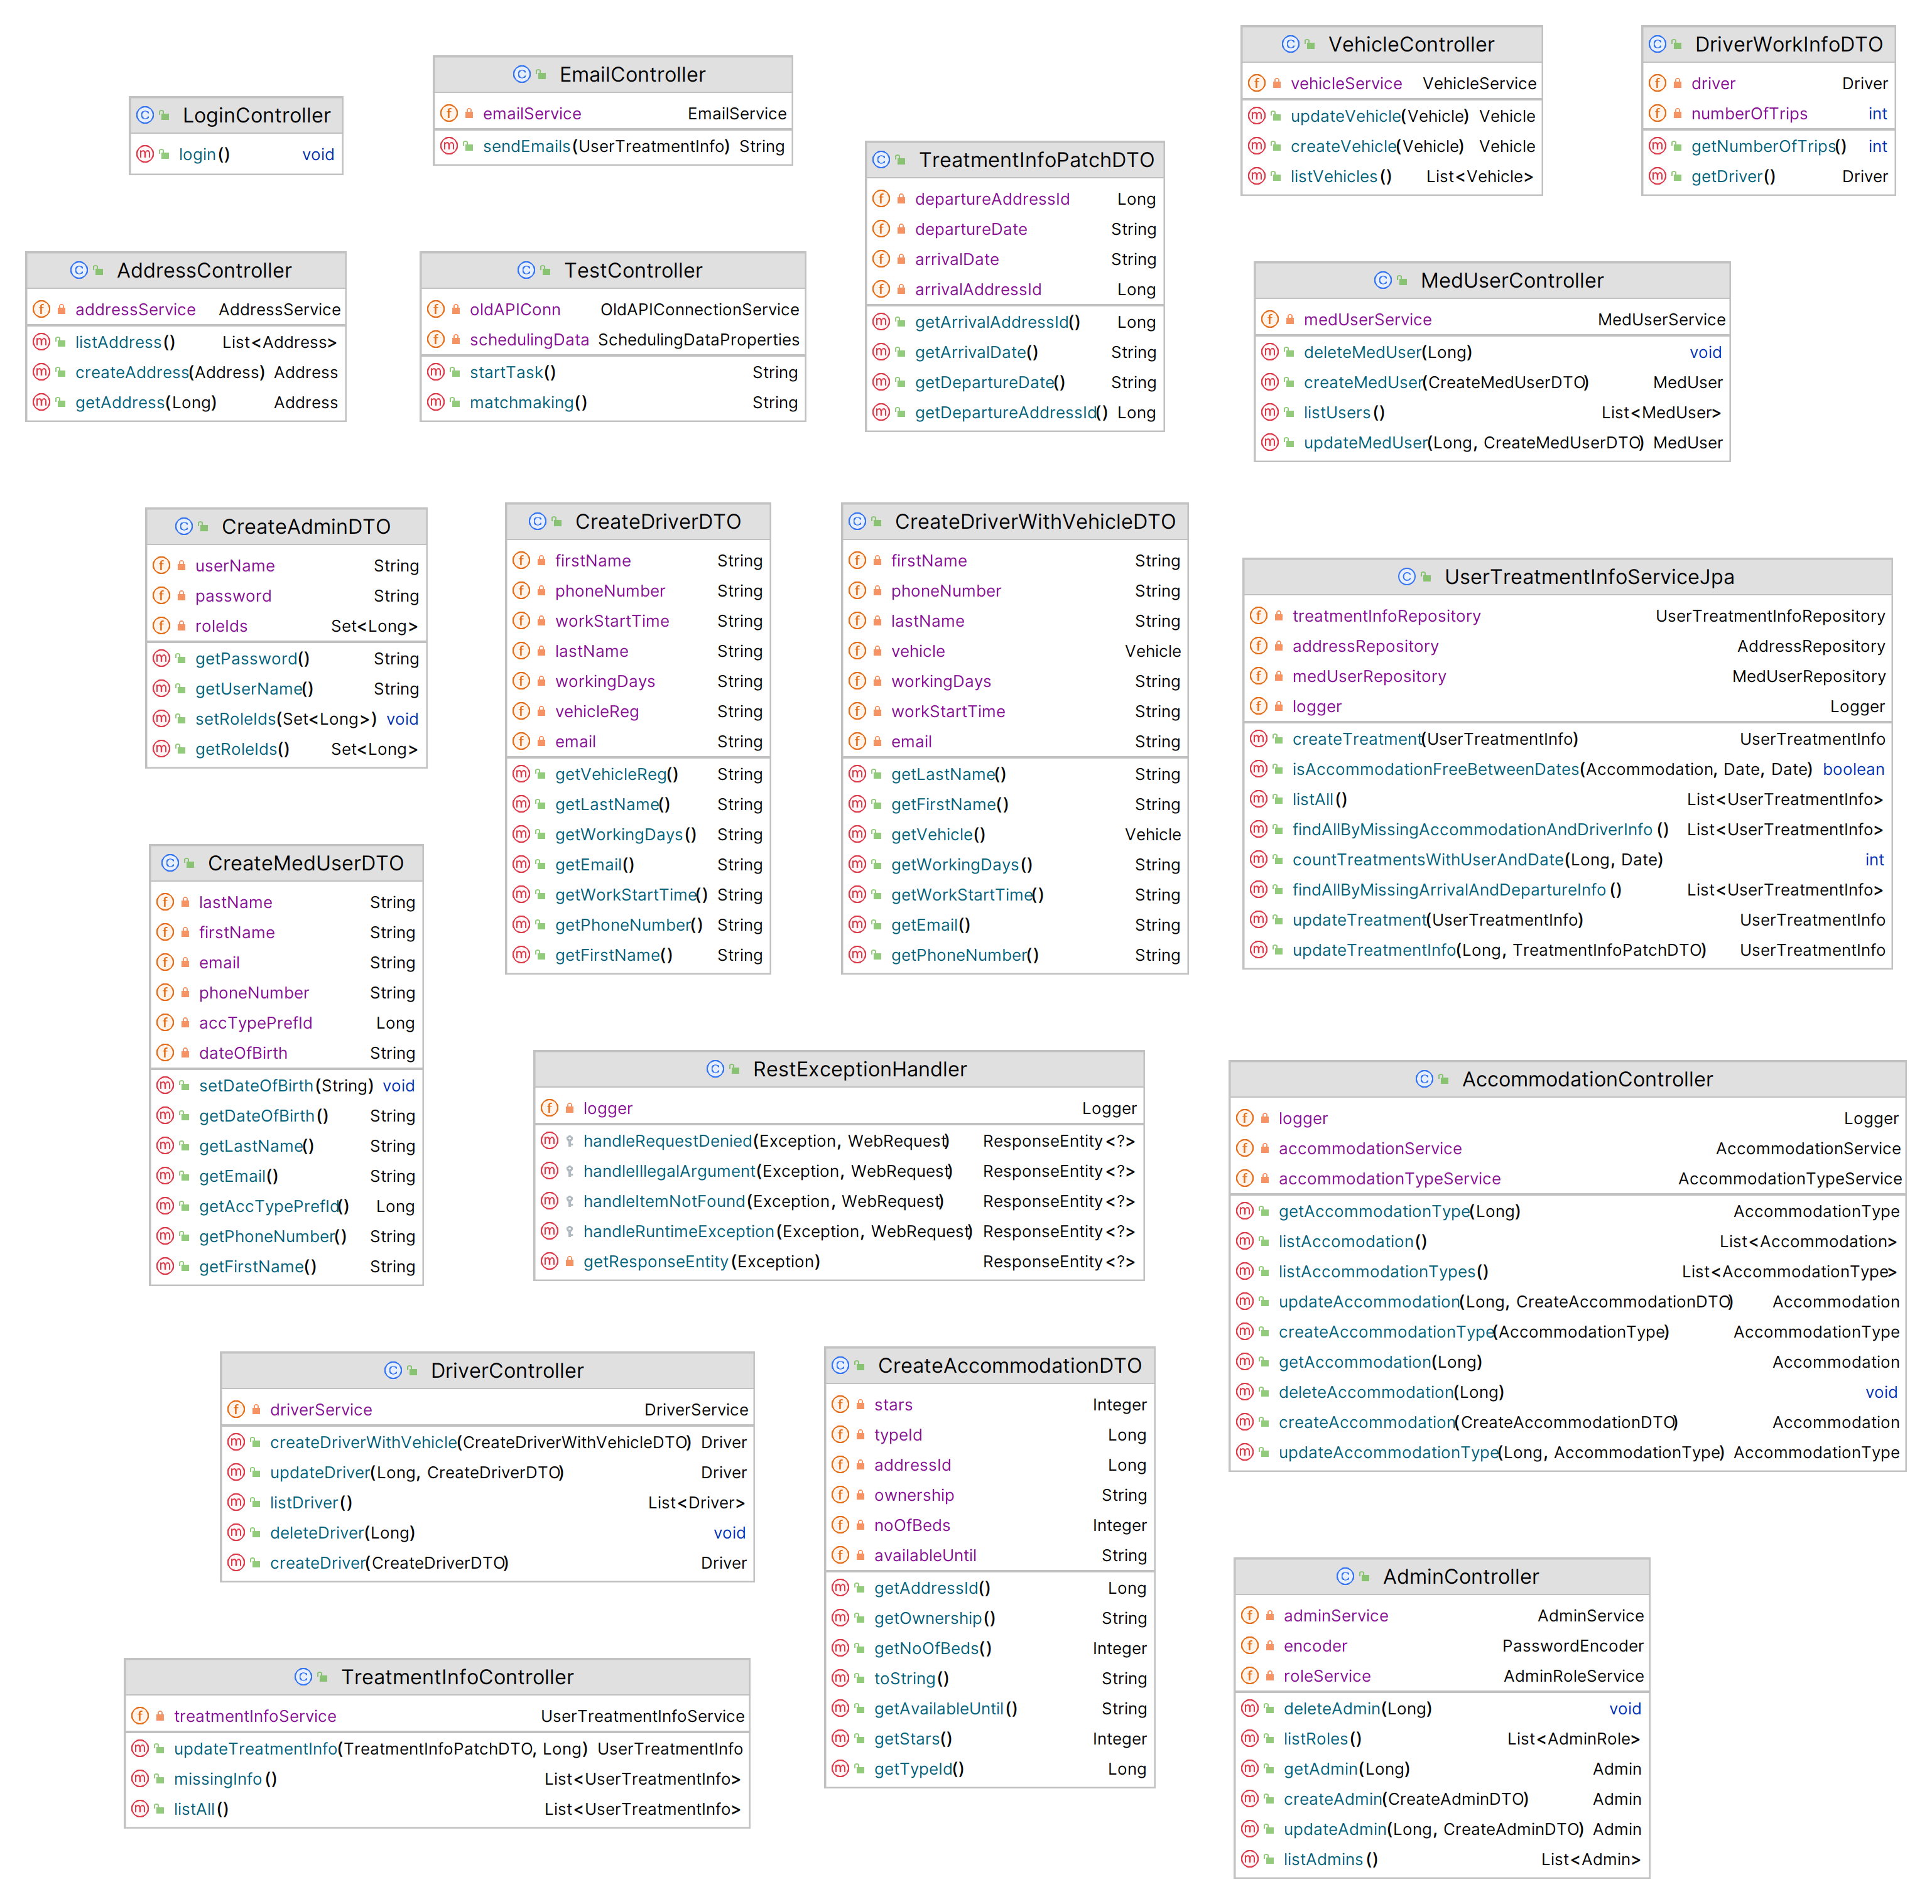
\includegraphics[width=\textwidth]{slike/rest.PNG}
				\caption{Dijagram razreda - Controller}
				\label{restDiagram}
			\end{figure}
			
			{Navedene klase nasljeđuju REST Controller koji je zadužen za rukovanje HTTP zahtjevima i za pružanje odgovarajućih odgovora. REST Controller vraća podatke u JSON formatu. \\ 
			CreateAdminDTO je \textit{Data transfer Object} koji je zadužen za stvaranje administratora. \textit{DTO} služi za transfer podataka između slojeva aplikacije, pogotovo između klijenta i servera. \\
			AdminUserDetailsService je \textit{Spring service} komponenta koja služi za baratanje detaljima administratora tijekom prijave i prilagođavanje korisničkih detalja na temelju odgovarajućih uloga i vjerodajnica, te osiguravanje sigurnosti}\\
			
			\begin{figure}[H]
				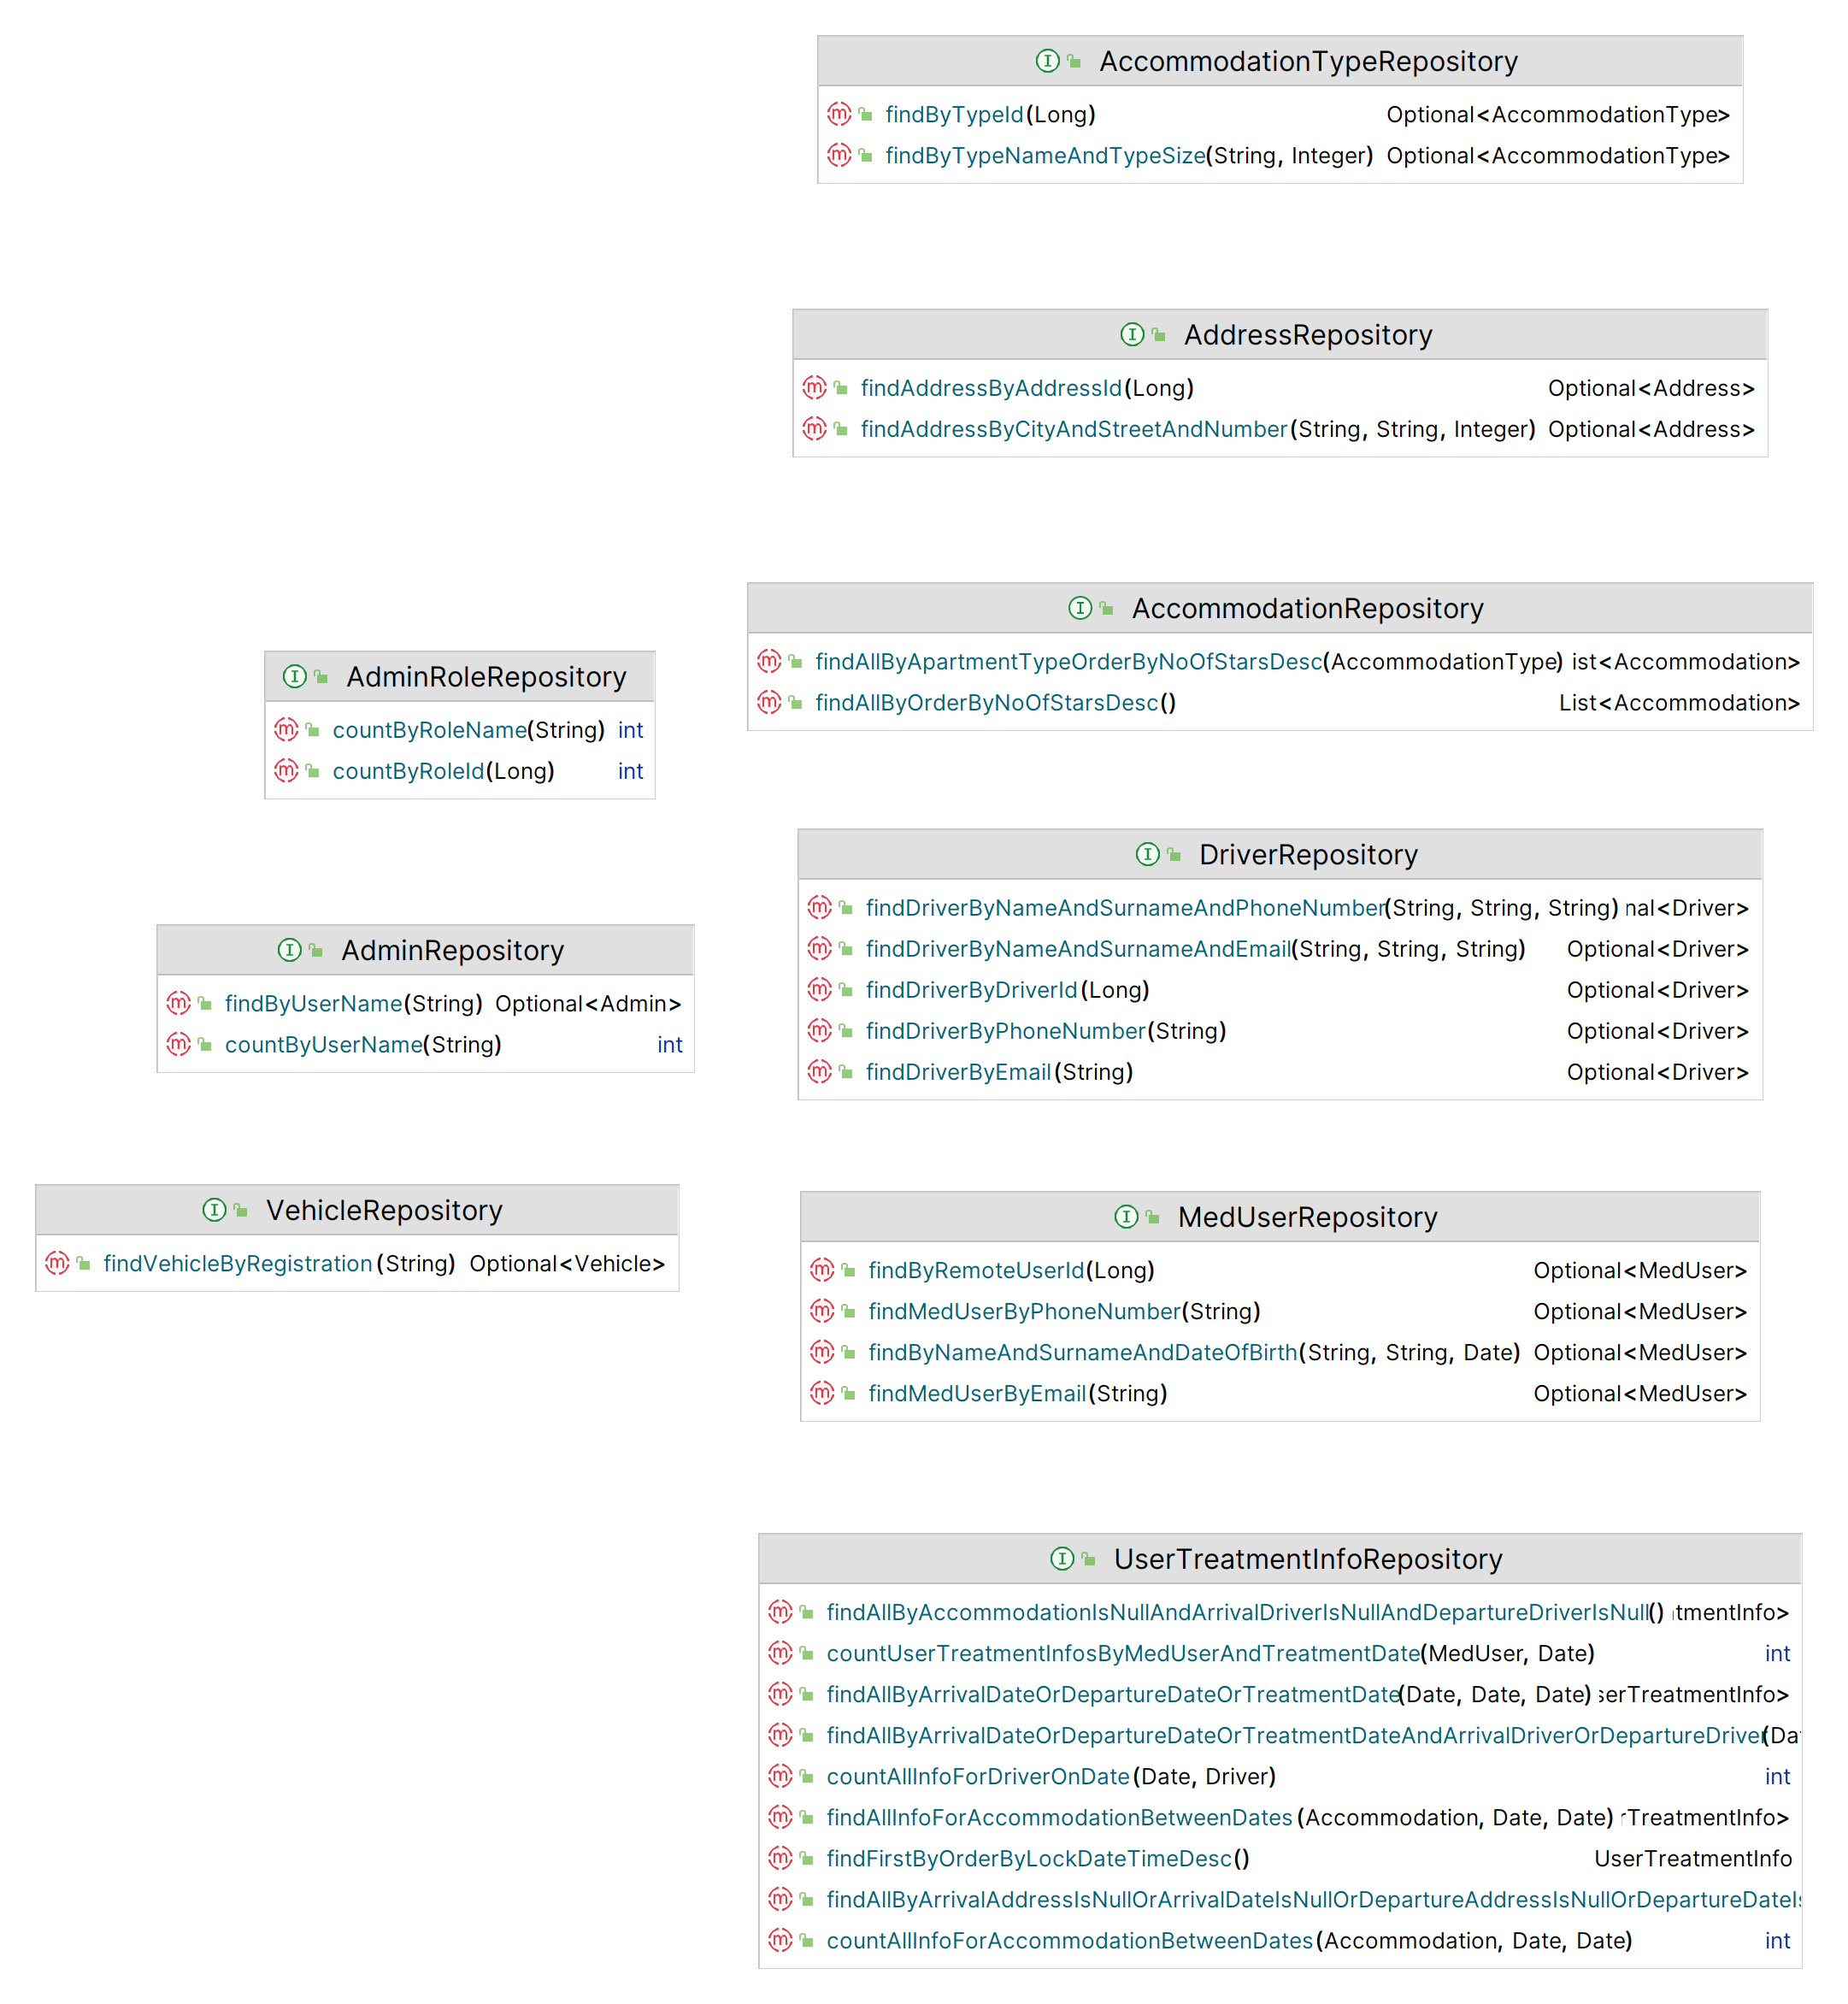
\includegraphics[width=\textwidth]{slike/dao.PNG}
				\caption{Dijagram razreda - Repository}
				\label{repositoryDiagram}
			\end{figure}
			
			{Navedena sučelja nasljeđuju \textit{JPARepository} koji pruža generičke metode za operacije s podatcima, poput spremanja, ažuriranja, brisanja i slično.}\\
			
			\begin{figure}[H]
				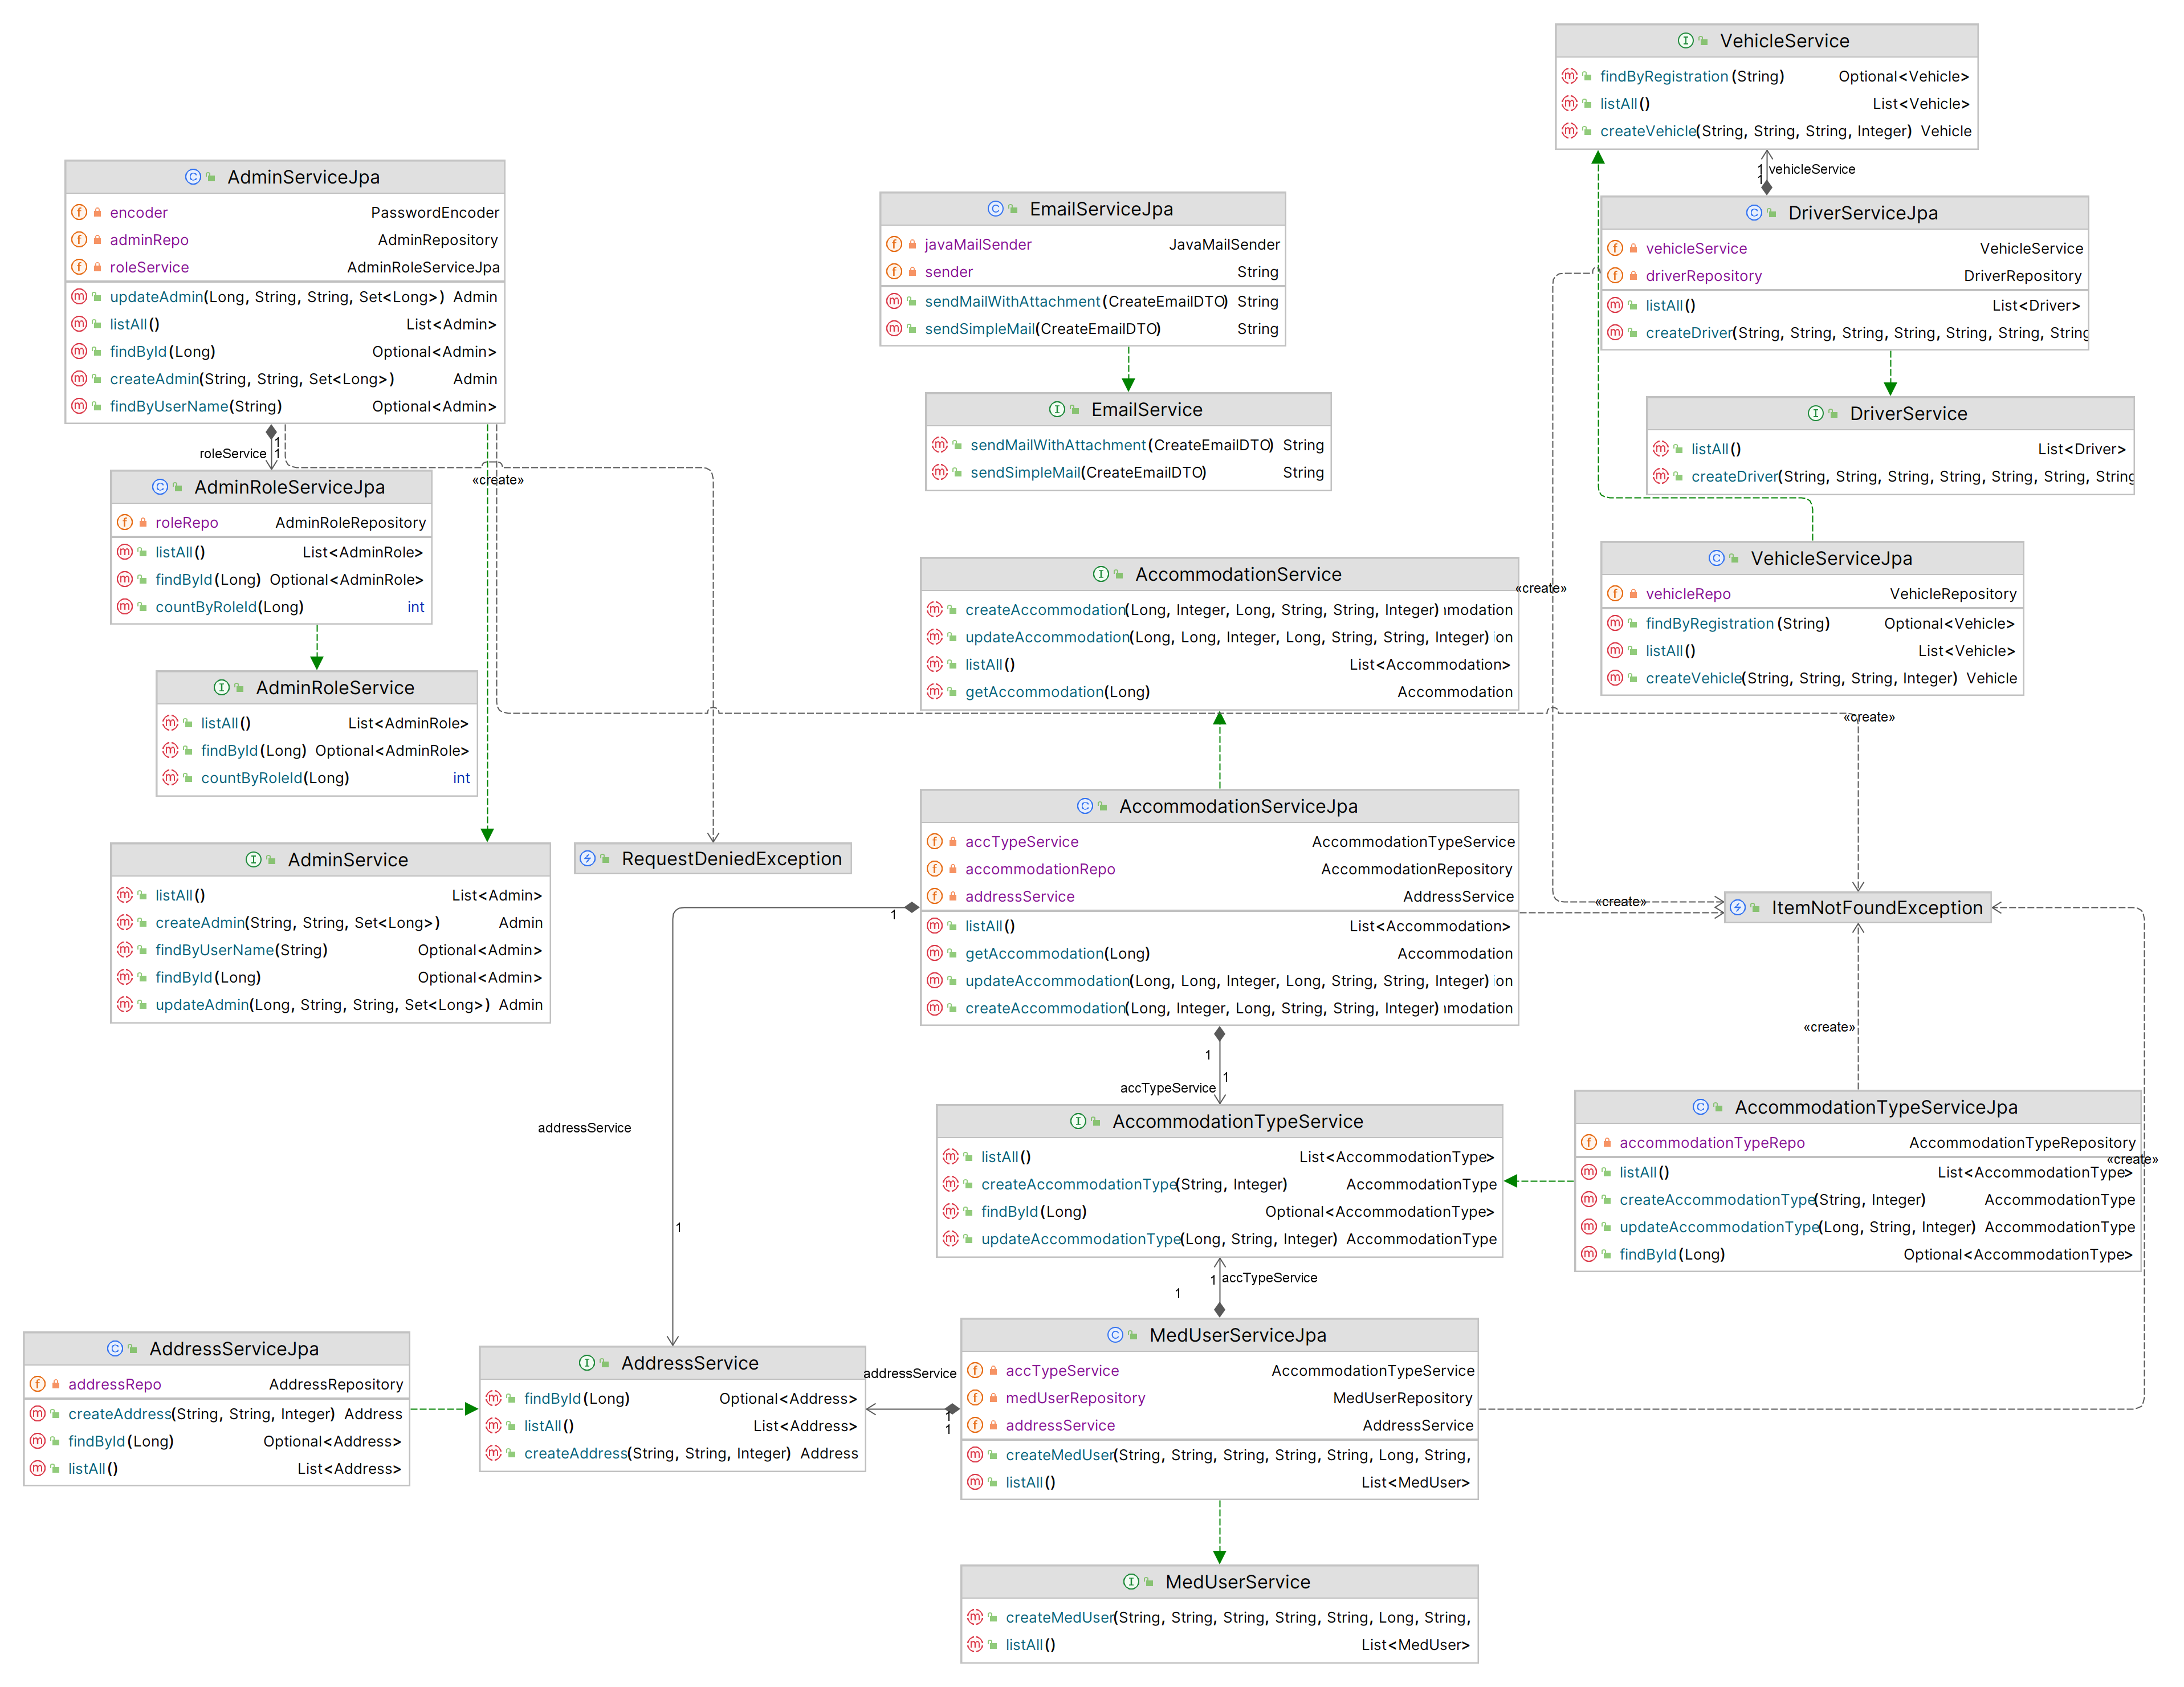
\includegraphics[width=\textwidth]{slike/service.PNG}
				\caption{Dijagram razreda - Service}
				\label{serviceDiagram}
			\end{figure}
			
			{Navedene \textit{Service} klase su \textit{Spring Service} klase, sadrže poslovnu logiku aplikacije, tj. odgovorni su za obradu podataka, implementaciju algoritama itd. Ponašaju se kao sloj između \textit{Controllera} i \textit{Repositoryja}.\\
			\textit{AdminService} sadrži metodu \textit{createAdmin} za stvaranje administratora. Postoji provjera raznih svojstava, poput duljine lozinke, duljine nadimka, postoji li već neki administrator s tim nadimkom, postojanje navedenih uloga itd. Ako je sve uspješno sprema se novi administrator u \textit{AdminRepository}.}\\
			
			\begin{figure}[H]
				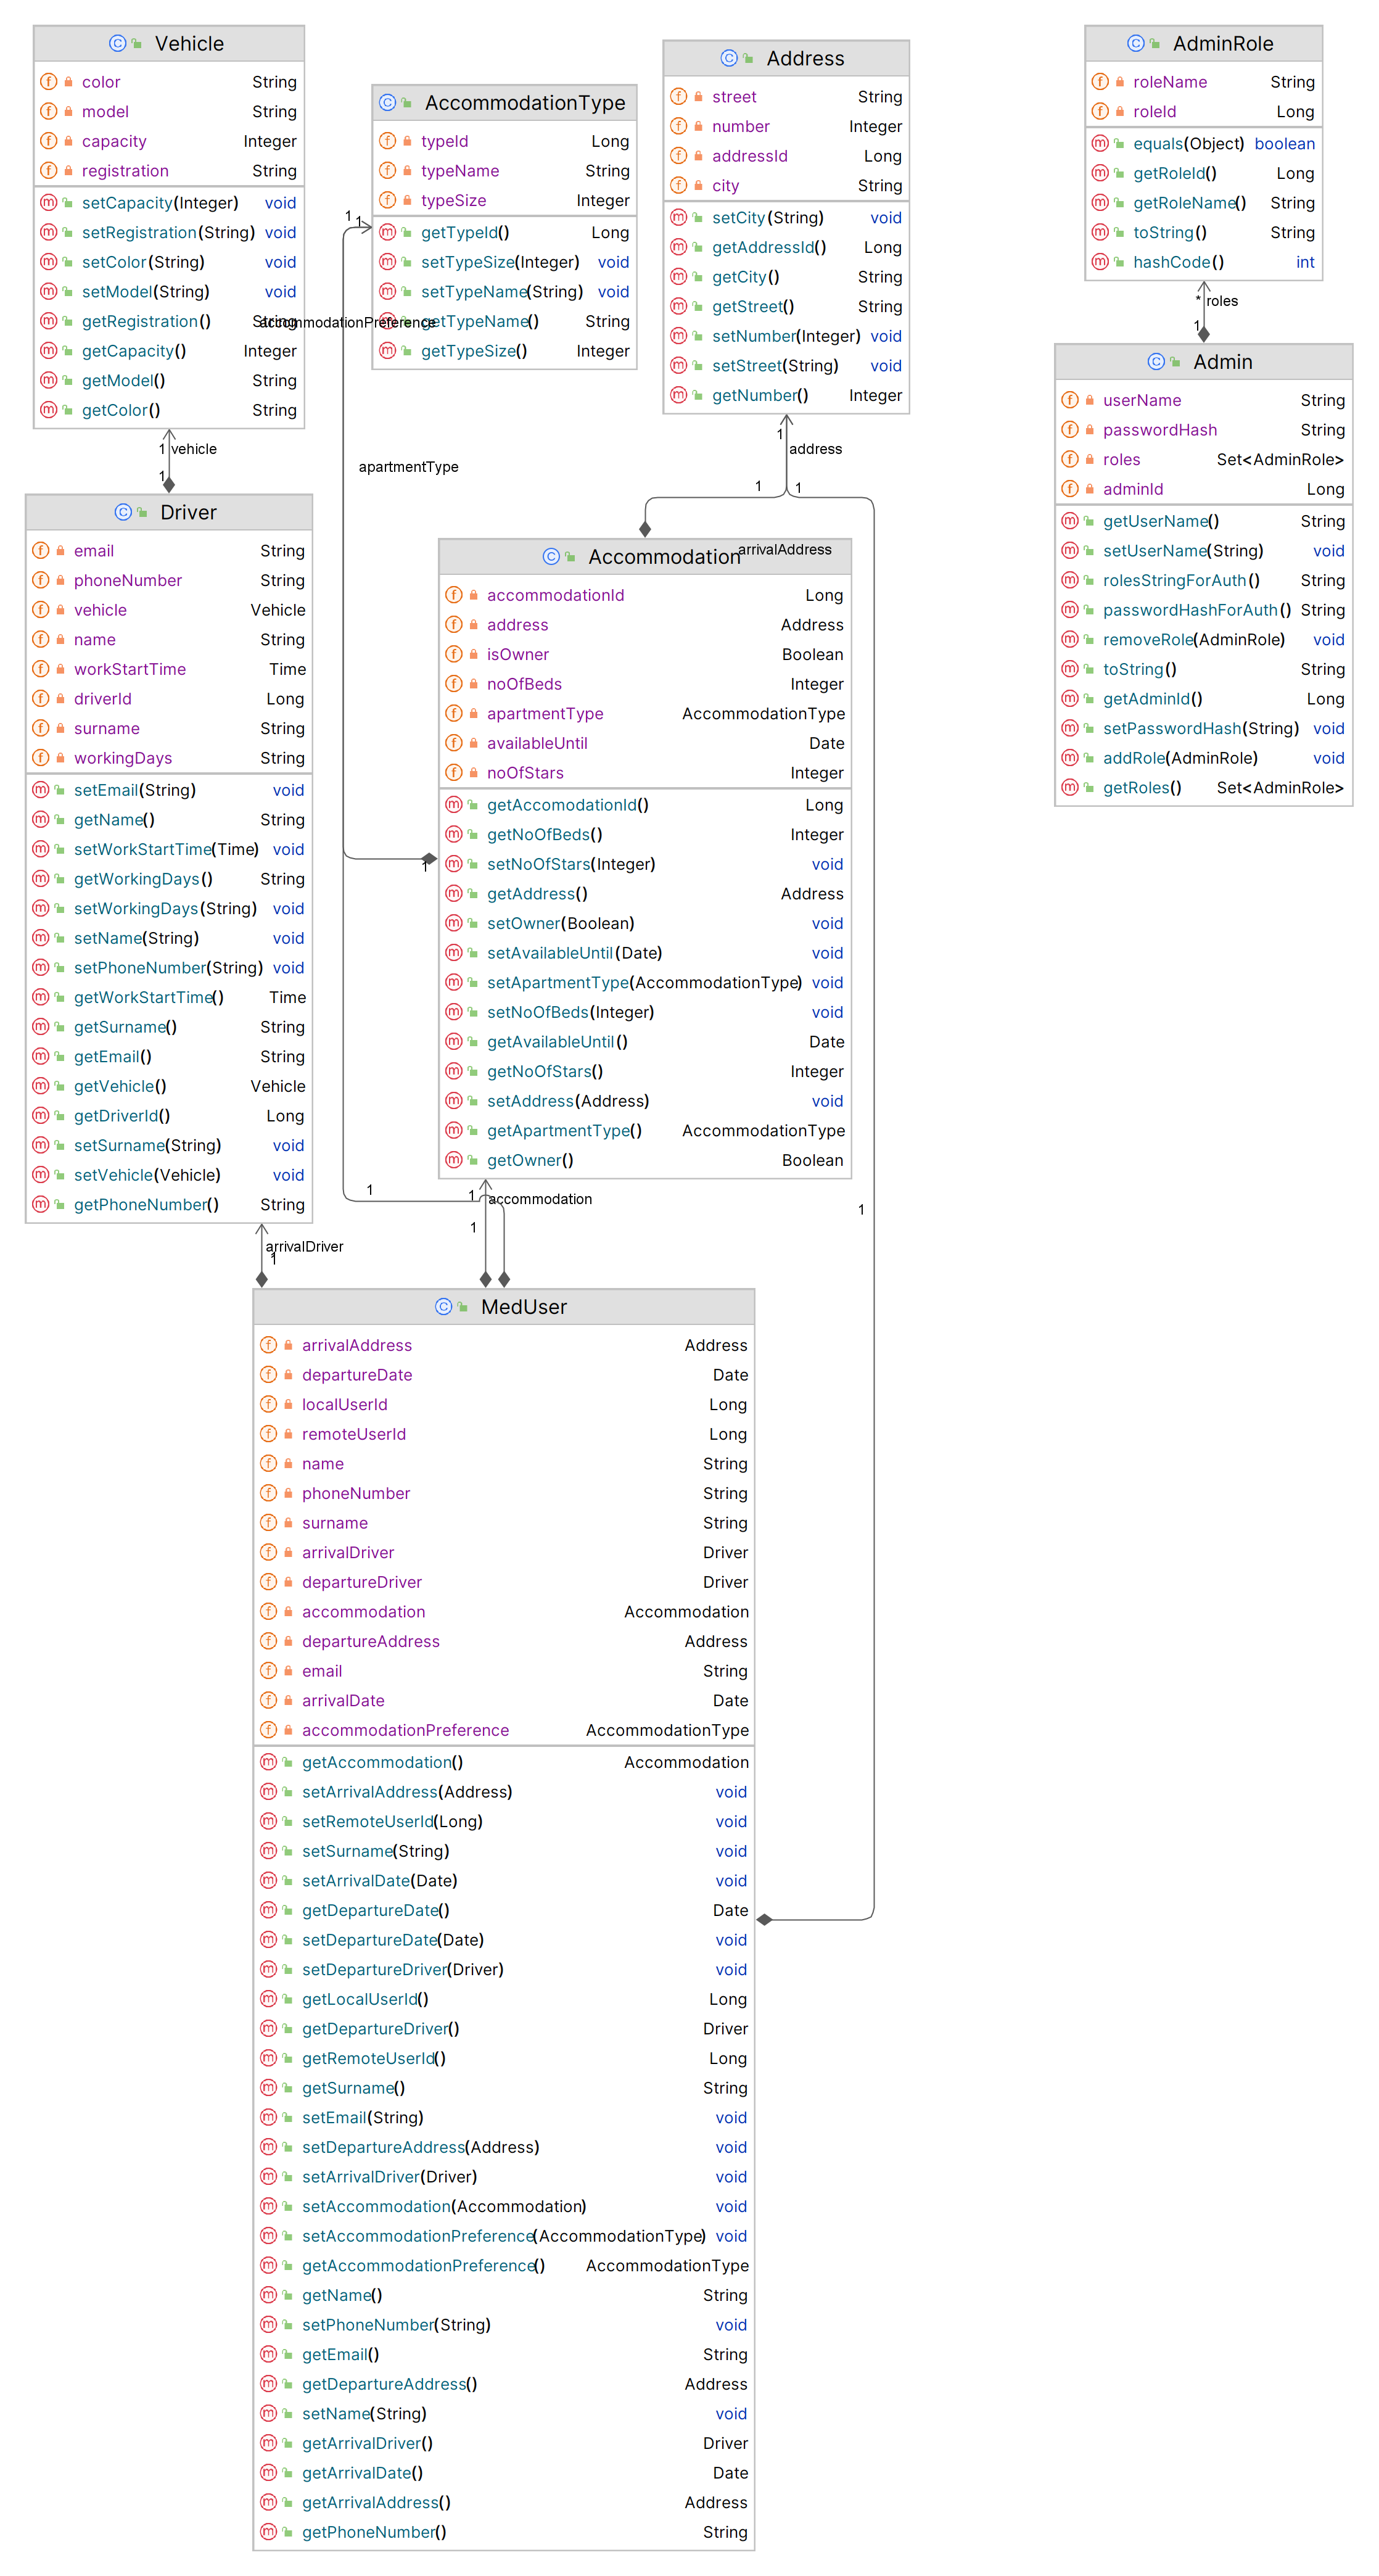
\includegraphics[width=\textwidth]{slike/domain.PNG}
				\caption{Dijagram razreda - Models}
				\label{domainDiagram}
			\end{figure}
			
			{Modeli predstavljaju strukturu baze podataka u našoj aplikaciji. Tako imamo klase: \textit{Admin, MedUser, Accomomodation te Transport} sa svojim privatnim atributima te javnim metodama. Tako na primjer \textit{Admin} ima svoj ID, nadimak, ime te pripadajuće uloge, koje mogu biti smještajni administrator(ima najveće ovlasti), korisnički administrator te prijevozni administrator, što je sadržano u enumeraciji \textit{AdminRole}. \textit{Accommodation} i \textit{Transport} sadrže sve podatke vezane uz smještaj, odnosno prijevoz, a \textit{MedUser} sadrži sve potrebno za definiranje korisnika medicinskih usluga. }\\
			
			
			
			\textbf{\textit{dio 2. revizije}}\\			
			
			\textit{Prilikom druge predaje projekta dijagram razreda i opisi moraju odgovarati stvarnom stanju implementacije}
			
			
			
			\eject
		
		\section{Dijagram stanja}
			
			
			\textbf{\textit{dio 2. revizije}}\\
			
			\textit{Potrebno je priložiti dijagram stanja i opisati ga. Dovoljan je jedan dijagram stanja koji prikazuje \textbf{značajan dio funkcionalnosti} sustava. Na primjer, stanja korisničkog sučelja i tijek korištenja neke ključne funkcionalnosti jesu značajan dio sustava, a registracija i prijava nisu. }
			
			
			\eject 
		
		\section{Dijagram aktivnosti}
			
			\textbf{\textit{dio 2. revizije}}\\
			
			 \textit{Potrebno je priložiti dijagram aktivnosti s pripadajućim opisom. Dijagram aktivnosti treba prikazivati značajan dio sustava.}
			
			\eject
		\section{Dijagram komponenti}
		
			\textbf{\textit{dio 2. revizije}}\\
		
			 \textit{Potrebno je priložiti dijagram komponenti s pripadajućim opisom. Dijagram komponenti treba prikazivati strukturu cijele aplikacije.}